\chapter{Save Page}

The Save Page is used to save track data from the Internal Sequencer, Machinedrum or AnalogFour to  specific slots in the current row of the Grid.\\
\\
There are three different save modes available:
\begin{itemize}
    \item SEQ: Save internal sequencer data and MD sound data.
    \item MD: Copy MD Sequencer data. Save MD sequencer data and MD sound data.
    \item MERGE: Merge MD Sequencer data with internal sequencer. Save sequencer data and MD sound data.
\end{itemize}
MD's Master Effects settings are also saved with each MD Track.
\textit{For technical reasons, MD and MERGE modes are only available when the sequencer playback is stopped.}
\\
\\The Save page is also used to save A4 tracks. When an A4 track is saved, the Sound Settings for the chosen track together with the internal sequencer data are stored together. Save mode has no effect here.

%\fbox{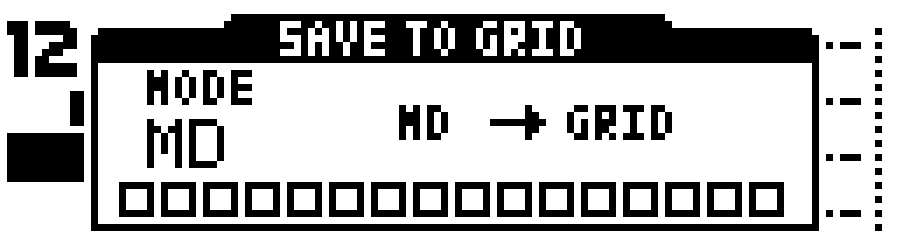
\includegraphics[scale=.40]{save_page.png}}\\

\screenshot{save_to_grid.png}

\textit{The Save Page is accessible from the GridPage by pressing the  \textbf{[Save]} function button.}

\encodersbuttons{Mode}{--}{--}{--}{cancels the save.}{--}{--}{save all tracks.}

\section{Saving Individual Tracks}
The Save Page uses the Trigger Interface to specify which tracks are to be saved. Pressing multiple trigger buttons on the MD and then releasing them will cause the selected tracks to be stored in the corresponding slots of the current row.

Similary, notes C -> F allow saving Analog4 tracks 1 to 4.
\section{Store a pattern/row:}
To save an entire pattern/row press \textbf{[Shift2]} from within the Save Page. All A4 sounds or external sequencer data will also be saved.



